\chapter{树}
  \begin{Def}
    连通且无圈的无向图称为无向树,简称{\bfseries树}。 一个没有圈的无向图
    称为无向森林,简称{\bfseries森林}。
  \end{Def}

  \begin{Ex}
  设$G=(V,E)$是一个$(p,q)$图,试证下列各命题等价:
  \begin{enumerate}
  \item $G$是树;
  \item $G$的任两个不同顶点间有唯一的一条路联结;
  \item $G$是连通的且去掉任意一条边则得到一个不连通的图;
  \item $G$是连通的且$q = p - 1$;
  \item $G$中无圈且$q = p - 1$;
  \item $G$中无圈且$G$中任意两个不邻接的顶点间加一条边则得到一个含有圈的图。
  \end{enumerate}
  \end{Ex}
  \begin{Ex}
  下列图为树的是\underline{$\quad\quad$}。
\end{Ex}

  \vspace{0.5cm}

  A.
    \begin{minipage}{0.18\linewidth}
    \centering
    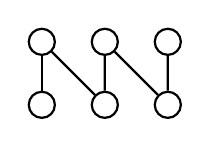
\begin{tikzpicture}[auto,
    specification/.style ={circle, draw, thick}, scale = 0.8]
   \node[specification] (A)  at (0,0)  {};
   \node[specification] (B)  at (1,0)  {};
   \node[specification] (C)  at (2,0)  {};
   \node[specification] (D)  at (0,1)  {};
   \node[specification] (E)  at (1,1)  {};
   \node[specification] (F)  at (2,1)  {};

   \draw[thick] (A) to  (D);
   \draw[thick] (B) to  (E);
   \draw[thick] (C) to  (F);
   \draw[thick] (B) to  (D);
   \draw[thick] (C) to  (E);
 \end{tikzpicture}
\end{minipage}\hfill
  B.
    \begin{minipage}{0.18\linewidth}
      \centering
          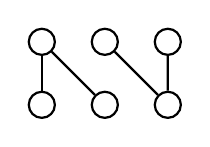
\begin{tikzpicture}[auto,
    specification/.style ={circle, draw, thick}, scale = 0.8]
   \node[specification] (A)  at (0,0)  {};
   \node[specification] (B)  at (1,0)  {};
   \node[specification] (C)  at (2,0)  {};
   \node[specification] (D)  at (0,1)  {};
   \node[specification] (E)  at (1,1)  {};
   \node[specification] (F)  at (2,1)  {};

   \draw[thick] (A) to  (D);
   \draw[thick] (C) to  (F);
   \draw[thick] (B) to  (D);
   \draw[thick] (C) to  (E);
 \end{tikzpicture}

\end{minipage}\hfill
      C.
    \begin{minipage}{0.18\linewidth}
      \centering
          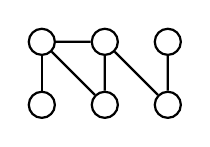
\begin{tikzpicture}[auto,
    specification/.style ={circle, draw, thick}, scale = 0.8]
   \node[specification] (A)  at (0,0)  {};
   \node[specification] (B)  at (1,0)  {};
   \node[specification] (C)  at (2,0)  {};
   \node[specification] (D)  at (0,1)  {};
   \node[specification] (E)  at (1,1)  {};
   \node[specification] (F)  at (2,1)  {};

   \draw[thick] (A) to  (D);
   \draw[thick] (B) to  (E);
   \draw[thick] (C) to  (F);
   \draw[thick] (B) to  (D);
   \draw[thick] (C) to  (E);
   \draw[thick] (D) to  (E);
 \end{tikzpicture}

\end{minipage}\hfill
      D.
    \begin{minipage}{0.18\linewidth}
      \centering
          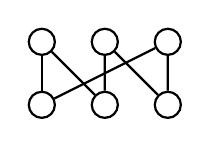
\begin{tikzpicture}[auto,
    specification/.style ={circle, draw, thick}, scale = 0.8]
   \node[specification] (A)  at (0,0)  {};
   \node[specification] (B)  at (1,0)  {};
   \node[specification] (C)  at (2,0)  {};
   \node[specification] (D)  at (0,1)  {};
   \node[specification] (E)  at (1,1)  {};
   \node[specification] (F)  at (2,1)  {};

   \draw[thick] (A) to  (D);
   \draw[thick] (B) to  (E);
   \draw[thick] (C) to  (F);
   \draw[thick] (B) to  (D);
   \draw[thick] (C) to  (E);
   \draw[thick] (A) to  (F);

 \end{tikzpicture}

\end{minipage}


\begin{Ex}
  下列图为森林的是\underline{$\quad\quad$}。
\end{Ex}

  \vspace{0.5cm}

  A.
    \begin{minipage}{0.18\linewidth}
      \centering
          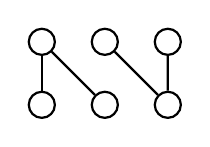
\begin{tikzpicture}[auto,
    specification/.style ={circle, draw, thick}, scale = 0.8]
   \node[specification] (A)  at (0,0)  {};
   \node[specification] (B)  at (1,0)  {};
   \node[specification] (C)  at (2,0)  {};
   \node[specification] (D)  at (0,1)  {};
   \node[specification] (E)  at (1,1)  {};
   \node[specification] (F)  at (2,1)  {};

   \draw[thick] (A) to  (D);
   \draw[thick] (C) to  (F);
   \draw[thick] (B) to  (D);
   \draw[thick] (C) to  (E);
 \end{tikzpicture}

\end{minipage}\hfill  
  B.
    \begin{minipage}{0.18\linewidth}
      \centering
          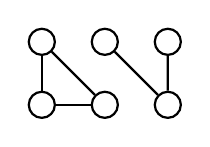
\begin{tikzpicture}[auto,
    specification/.style ={circle, draw, thick}, scale = 0.8]
   \node[specification] (A)  at (0,0)  {};
   \node[specification] (B)  at (1,0)  {};
   \node[specification] (C)  at (2,0)  {};
   \node[specification] (D)  at (0,1)  {};
   \node[specification] (E)  at (1,1)  {};
   \node[specification] (F)  at (2,1)  {};

   \draw[thick] (A) to  (D);
   \draw[thick] (C) to  (F);
   \draw[thick] (B) to  (D);
   \draw[thick] (C) to  (E);
   \draw[thick] (A) to  (B);
   
 \end{tikzpicture}

\end{minipage}\hfill
C.
\begin{minipage}{0.18\linewidth}
      \centering
          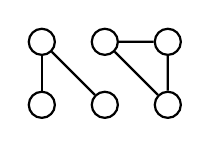
\begin{tikzpicture}[auto,
    specification/.style ={circle, draw, thick}, scale = 0.8]
   \node[specification] (A)  at (0,0)  {};
   \node[specification] (B)  at (1,0)  {};
   \node[specification] (C)  at (2,0)  {};
   \node[specification] (D)  at (0,1)  {};
   \node[specification] (E)  at (1,1)  {};
   \node[specification] (F)  at (2,1)  {};

   \draw[thick] (A) to  (D);
   \draw[thick] (C) to  (F);
   \draw[thick] (B) to  (D);
   \draw[thick] (C) to  (E);
      \draw[thick] (E) to  (F);

 \end{tikzpicture}

\end{minipage}\hfill
D.
    \begin{minipage}{0.18\linewidth}
      \centering
          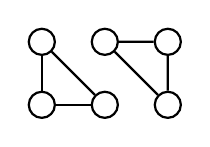
\begin{tikzpicture}[auto,
    specification/.style ={circle, draw, thick}, scale = 0.8]
   \node[specification] (A)  at (0,0)  {};
   \node[specification] (B)  at (1,0)  {};
   \node[specification] (C)  at (2,0)  {};
   \node[specification] (D)  at (0,1)  {};
   \node[specification] (E)  at (1,1)  {};
   \node[specification] (F)  at (2,1)  {};

   \draw[thick] (A) to  (D);
   \draw[thick] (C) to  (F);
   \draw[thick] (B) to  (D);
   \draw[thick] (C) to  (E);
   \draw[thick] (A) to  (B);
   \draw[thick] (E) to  (F);


 \end{tikzpicture}

\end{minipage}

%%% Local Variables:
%%% mode: latex
%%% TeX-master: "book"
%%% End:
